%----------------------------------------------------------------------------
%
%	This template was created by
%		Christian Krieg <christian.krieg@alumni.tuwien.ac.at>
%
%	April 2018
%
%----------------------------------------------------------------------------
%
\documentclass[%
	a4paper,
]
{article}
%
%----------------------------------------------------------------------------
%
% Institution
%
%\institution{Institute of Computer Technology}
%
%----------------------------------------------------------------------------
%
% Use the 'Libertine' font type
%
%\usepackage{libertine}
\usepackage[T1]{fontenc}
\usepackage[utf8]{inputenc}
%
%----------------------------------------------------------------------------
%
% Set page margins
%
\usepackage{geometry}
\geometry{%
	left   = 2cm,
	right  = 2cm,
	top    = 2cm,
	bottom = 2cm
}
%
%----------------------------------------------------------------------------
%
% Set line spacing
%
\usepackage{setspace}
\setstretch{1}
%
%----------------------------------------------------------------------------
%
% Settings for hyperlinks
%
\usepackage{hyperref}
\hypersetup{%
	colorlinks = true,
	allcolors  = blue,
}
%
%----------------------------------------------------------------------------
%
% Use colors
%
\usepackage{xcolor}
\usepackage{colortbl}
%
%----------------------------------------------------------------------------
%
% Define a TODO and a DONE command
%
\newcommand{\todo}[1]{\textcolor{red}{#1}}
\newcommand{\done}[1]{}
%
%----------------------------------------------------------------------------
%
% Use glossaries
%
\usepackage{glossaries}
\makeglossaries
%
% Glossary entries
%
\newglossaryentry{fpga}{
	name = {FPGA},
	description = {Field-programmable gate array},
	text = {FPGA},
	first = {field-programmable gate array (FPGA)},
	plural = {FPGAs},
	firstplural = {field-programmable gate arrays (FPGAs)},
}
%
\newglossaryentry{trng}{
	name = {TRNG},
	description = {True-random number generator},
	text = {TRNG},
	first = {true-random number generator (TRNG)},
	plural = {TRNGs},
	firstplural = {true-random number generators (TRNGs)},
}
%
\newglossaryentry{bcd}{
  name={BCD},
  description={Binary-coded decimal},
  text={BCD},
  first={binary-coded decimal (BCD)},
}
%
\newglossaryentry{hdl}{
  name={HDL},
  description={Hardware description language},
  text={HDL},
  first={hardware description language (HDL)},
  plural={HDLs},
  firstplural={hardware description languages (HDLs)},
}
%
\newglossaryentry{ip}{
  name={IP},
  description={Intellectual property},
  text={IP},
  first={intellectual property (IP)},
}
%
\newglossaryentry{3pip}{
  name={3PIP},
  description={Third-party intellectual property},
  text={3PIP},
  first={third-party intellectual property (3PIP)},
}
%
\newglossaryentry{dsp}{
  name={DSP},
  description={Digital signal processor},
  text={DSP},
  first={digital signal processor (DSP)},
  plural={DSPs},
  firstplural={digital signal processors (DSPs)},
}
%
%\newglossaryentry{}{
%  name={},
%  description={},
%  text={},
%  first={},
%  plural={},
%  firstplural={},
%}
%
%----------------------------------------------------------------------------
%
% Settings for citations and the bibliography
%
\usepackage[%
	backend     = biber,
	maxbibnames = 99,
	autocite    = footnote,
	citestyle   = verbose-ibid,
	firstinits=true,
]{biblatex}
\bibliography{bib/report}
%
%----------------------------------------------------------------------------
%
%	TikZ -- TikZ ist kein Zeichenprogramm
%
\usepackage{tikz}
\usepackage{tikz-timing}
\usepackage{etoolbox}
\usetikzlibrary{mindmap}
\usetikzlibrary{shapes}
\usetikzlibrary{arrows}
\usetikzlibrary{decorations}
\usetikzlibrary{shapes.symbols}
\usetikzlibrary{shapes.geometric}
\usetikzlibrary{shapes.multipart}
\usetikzlibrary{positioning}
\usetikzlibrary{patterns}
\usetikzlibrary{calc}
\usetikzlibrary{scopes}         % cf. pgfmanual p.66
\usetikzlibrary{chains}         % cf. pgfmanual p.284
\usetikzlibrary{fit}
\usetikzlibrary{matrix}
\usetikzlibrary{decorations}
\usetikzlibrary{circuits.logic}
\usetikzlibrary{circuits.logic.IEC}
\usetikzlibrary{shapes.gates.logic.IEC}
\usetikzlibrary{circuits.logic.US}
\usetikzlibrary{shapes.gates.logic.US}
\usetikzlibrary{circuits.ee}
\usetikzlibrary{circuits.ee.IEC}
\usetikzlibrary{backgrounds}
\usetikzlibrary{automata}
\usetikzlibrary{intersections}
\usetikzlibrary{plotmarks}
\usepgflibrary{fpu}
\usetikzlibrary{decorations.pathreplacing}
%
%----------------------------------------------------------------------------
%
% TikZ shapes
%  
	\input{lib/tikz/dff}
%
%----------------------------------------------------------------------------
%
% Use AMS math fonts
%
\usepackage{amsfonts}
\usepackage[sans]{dsfont}
%
%----------------------------------------------------------------------------
%
% Use multiple figures in one float
%
\usepackage{subcaption}
%
%----------------------------------------------------------------------------
%
% Use dummy text
%
\usepackage{lipsum}
%
%----------------------------------------------------------------------------
%
% Use extended list environments (e.g., 'inparaenum')
%
\usepackage{paralist}
%
%----------------------------------------------------------------------------
%
% Use listings
%
\usepackage{listings}

\lstdefinestyle{vhdl}
{
	language=VHDL,
  basicstyle=\linespread{1}\scriptsize\ttfamily\color{black},
  commentstyle=\scriptsize\itshape,
  escapeinside={(*@}{@*)},
  frame=single, numbers=left,
%  numbersep=5pt,
  xleftmargin=15pt,
  xrightmargin=5pt,
  numbersep=5pt,
  breaklines=true,
  moredelim=**[is][\ttfamily\bfseries\color{red}]{(*}{*)},
}

\lstdefinestyle{verilog}
{
	language=Verilog,
  basicstyle=\linespread{1}\scriptsize\ttfamily\color{black},
  commentstyle=\scriptsize\itshape,
  escapeinside={(*@}{@*)},
  frame=single, numbers=left,
%  numbersep=5pt,
  xleftmargin=15pt,
  xrightmargin=5pt,
  numbersep=5pt,
  breaklines=true,
  moredelim=**[is][\ttfamily\bfseries\color{red}]{(*}{*)},
}
%
%----------------------------------------------------------------------------
%
% Typeset pseudo code
%
\usepackage{syntax}
%
%----------------------------------------------------------------------------
%
% More options for boxes
%
\usepackage{realboxes}
%
% Command for vertical text in tabulars
%
\newcommand*\rot{\rotatebox{90}}
%
%----------------------------------------------------------------------------
%
% Use \textsubscript
%
\usepackage{fixltx2e}
%
%----------------------------------------------------------------------------
%
% More options for tabulars
%
\usepackage{array}
%
%----------------------------------------------------------------------------
%
% Use appendices
%
\usepackage[titletoc]{appendix}
%
%----------------------------------------------------------------------------
%
% Use the cleverref package -- Load this package as the very last!
%
\usepackage{cleveref}
%
%----------------------------------------------------------------------------
%
% Document body
%
\begin{document}
%
%----------------------------------------------------------------------------
%
\begin{titlepage}

	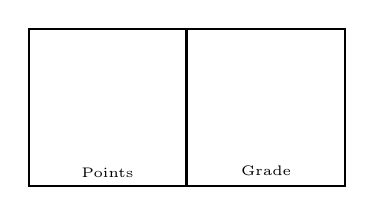
\begin{tikzpicture}[thick]
		\node (points) at (0,0) [draw,minimum size=2cm] {};
		\node (lbl-points) at (points.south) [anchor=south,font=\tiny] {Points};
		\node (grade) at (points.east) [draw,minimum size=2cm,anchor=west,
			outer sep=0] {};
		\node (lbl-grade) at (grade.south) [anchor=south,font=\tiny] {Grade};
	\end{tikzpicture}

	\begin{flushright}

		% Update this with your team number
		\huge\bfseries
		Team: - \\[1em]

		% Update this with your matriculation number, first name, second name
		\large
		1525864 Andreas Glinserer	\\
	
	\end{flushright}

	\vspace{5em}

	\begin{center}
		{\huge Digital Integrated Circuits Lab (LDIS)}\\[1em]
		{\Large 384.088, Summer Term 2019} \\[2em]
		{\large Supervisors:\\[.5em]
			Christian Krieg, David Radakovits, Axel Jantsch} \\[10em]

		{\Huge Task 1: Digital Thermometer}\\[10em]
	\end{center}


%	\begin{abstract}
%
%		Enter the abstract of your report here. An abstract summarizes your
%		entire work (i.e., problem statement, motivation, methodology, key
%		findings). It is a good strategy to write a first version of the abstract
%		when you start to work on your report. This gives you a good guideline
%		what to	put and what not to put into the report. Ideally, you re-write
%		the abstract once you finished your report, because only at this point
%		you have all the information available to create a good abstract.
%
%	\end{abstract}

\end{titlepage}
%
%----------------------------------------------------------------------------
%

\section{Problem statement}

The goal was to design a digital thermometer with the Nexys 4 DDR FPGA Board. To use was
one of the two temperature sensors on the board. One sensor is especially for measuring the 
temperature and to read out via i2c, while the other one is part of the accelerometer sensor
and is to read out with SPI. The samling rate of the sensor should be defined pre-synthesis.
The data then should go to an DSP part which was to be implemented as an moving average
filter. The filter width should be able to be changed during runtime. The output of the DSP should
be displayed on the 8 BCD segments on the board.

\begin{figure}[ht!]
	\centering
	\includegraphics[width=16cm]{fig/block}
	\caption{Block diagram of the system. Source: Original Task Description}
	\label{fig:block}
\end{figure}

\begin{figure}[ht!]
	\centering
	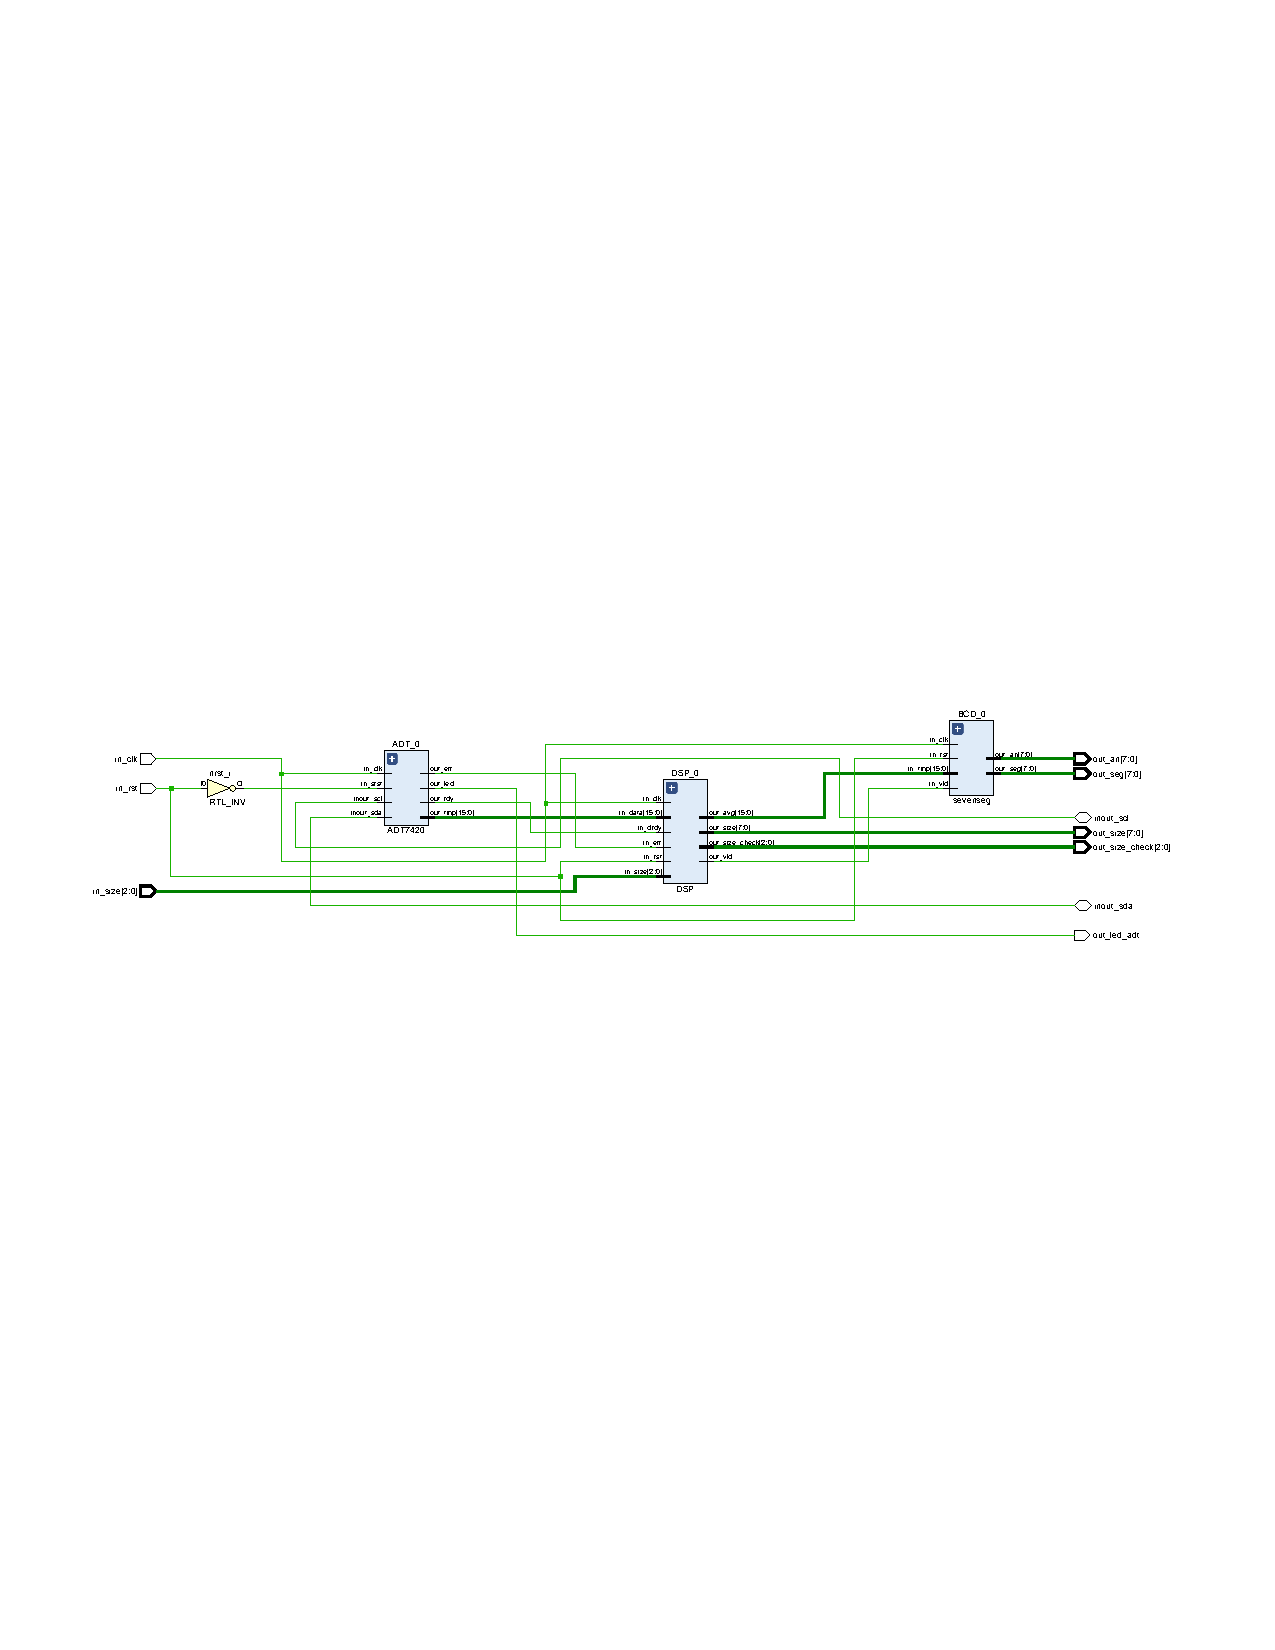
\includegraphics[width=16cm]{fig/schematic}
	\caption{Schematic of the system. Source: Vivado}
	\label{fig:block}
\end{figure}

\section {Implementation}
In this section I explain how i implemented a possible solution to the proposed problem. I choose
to use an active low reset for this task, which is the onboard switch with the name SW15.

\subsection{Sampling}
For the reading of the temperature i choose the onboard I2C-sensor. To get the values I
used the IP-core from the Nexys 4 DDR Demo which includes an readout of this sensor.
The sensor itself is an ADT7420 I2C temperature sensor. The output of the sampling part
consists of the out_data and the out_vld ports. The out_vld ports is high for the time of 
once clock cycle. It also has one LED, which toggles everytime valid data was retrieved.

\subsubsection{Changes of the IP}
The TWI Controller file was changed only in the way to use the ieee.numeric_std.all; library.
Other than that this file is original.

To the original readoutfiles were made some changes to get the wished functionality.
To get 16 bit readouts I added another init vector:

\lstset{style=vhdl, firstnumber=118}
\begin{lstlisting}
constant NO_OF_INIT_VECTORS : natural := 4; -- number of init vectors in TempSensInitMap
constant DATA_WIDTH : integer := 1 + 8 + 8; -- RD/WR bit + 1 byte register address + 1 byte data
constant ADDR_WIDTH : natural := natural(ceil(log(real(NO_OF_INIT_VECTORS), 2.0)));

type TempSensInitMap_type is 
	array (0 to NO_OF_INIT_VECTORS-1) of std_logic_vector(DATA_WIDTH-1 downto 0);
signal TempSensInitMap: TempSensInitMap_type := (
IRD & x"0B" & x"CB", -- Read ID R[0x0B]=0xCB
IWR & x"2F" & x"00", -- Reset R[0x2F]=don't care
IRD & x"0B" & x"CB", -- Read ID R[0x0B]=0xCB
IWR & x"03" & x"80"  -- configure it for 16bit
);
\end{lstlisting}

To get the sampling timing right i added an extra state in which the I2C waits.

\lstset{style=vhdl, firstnumber=101}
\begin{lstlisting}
constant SAMPLECNT : NATURAL := natural(ceil(real(clockfreq*1_000_000/Samples)))*2;

-- State Machine states definition
type state_type is (
	stIdle, -- Idle State
	stInitReg,  -- Send register address from the init vector
	stInitData, -- Send data byte from the init vector
	stRetry,    -- Retry state reached when there is a bus error, will retry RETRY_COUNT times
	stReadTempR,  -- Send temperature register address
	stReadTempD1, -- Read temperature MSB
	stReadTempD2, -- Read temperature LSB
	stError, -- Error state when reached when there is a bus error after a successful init; stays here until reset
	stWait  -- State to wait for the next sample
);
signal state, nstate : state_type;
\end{lstlisting}

The new state was also added to the ReadyFlag process:

\lstset{style=vhdl, firstnumber=252}
\begin{lstlisting}
----------------------------------------------------------------------------------
-- Ready Flag
----------------------------------------------------------------------------------  
ReadyFlag: process (in_clk)
begin
	if Rising_Edge(in_clk) then
		if (state = stIdle or state = stError) or state = stWait then
			fReady <= false;
		elsif (state = stReadTempD2 and twiDone = '1' and twiErr = '0') then
			fReady <= true;
		end if;
	end if;
end process;
\end{lstlisting}

In the OUTPUT_DECODE process another when statement got added.
\lstset{style=vhdl, firstnumber=349}
\begin{lstlisting}
when stWait =>
	null;
\end{lstlisting}

In the NEXT_STATE_DECODE process the stReadTempD2 state got changed and another state got added:
\lstset{style=vhdl, firstnumber=410}
\begin{lstlisting}
when stReadTempD2 =>
	if (twiDone = '1') then
		if (twiErr = '1') then
			nstate <= stError;
		else
			nstate <= stWait;
--                  nstate <= stReadTempR; -- old version
		end if;
	end if;
 
when stWait =>
	if waitSample = SAMPLECNT then
		nstate <= stReadTempR;
	end if;
\end{lstlisting}

And a whole new process got added in which the counting happens for the sampling rate:
\lstset{style=vhdl, firstnumber=265}
\begin{lstlisting}
---------------------------------------------------------------------------------- 
-- Sample counter wait               
----------------------------------------------------------------------------------  
SAMPLEWAIT : process(in_clk)                                       
begin                                                       
	if rising_edge(in_clk) then   
		if state = stWait then                       
			if waitSample = SAMPLECNT then             
				out_led <= led_helper; 
				led_helper <= not led_helper; 
			else 
				waitSample <= waitSample+1; 
			end if;                                                            

		else                                                                   
			waitSample <= 0;
		end if;                  
	end if;                 
end process;
\end{lstlisting}

\subsection{DSP}
The moving average is implemented as a state machine. The size of the filter window is determined
by the 3 switches SW2, SW1 and SW0. Each switch equals a number to the power of 2. 
SW0 = 1, SW1=2 and SW2=4. For example if SW2 is 
switched on and the others off then the size equals $2^{4}=16$. or if SW1 and SW2 are on then the
size equals $2^{2+1}=8$. It is done this way to make the divison for the mean value easier, since
divison by a number which is a power of two equals a bitshift to the right.

The formula of the mean averge is dependent on the size which gets choosen by the switches.

\begin{equation}
y = \sum_{i=0}^n x[i]
\end{equation}
Where $i$ represents the last value in the buffer. This way the mean average is causal but the mean
value is shifted if you print it against the original values.

I choose to implement it with a state machine. I also tried it with for loops but it took very
long to synthesize. The synthesizing time shrunk from greater than
25 minutes down to less than 7 minutes.

When the size gets changed the buffer gets set to zero. It then gets slowly refilled and the temperature
which gets sent to the BCD slowly increases, because it uses the fixed size for the division. 
It is done this way to show the working of the filter on the FPGA.

\subsection{Output}
The output part gets the averaged temperature. The hard part is to get from the binary value to a 
representation which fits on the BCD. One cannot just take the usual 4 bit approach for a segment 
because in the decimal system values only range from 0 to 9. So if the value would be an B in hex
one needs to subtract from the current position and add to the next position. This problem is solved
by using the double dabble algorithm (explanation on \href{https://en.wikipedia.org/wiki/Double_dabble}{Wikipedia} or \href{https://www.youtube.com/watch?v=eXIfZ1yKFlA}{Youtube}).

Since the BCD share the an anode contact there is also the need to multiplex the data which gets
to the corresponding outputs. This is done with the out_an outputs. It is also important to notice
that the active select anode is active low.

This is solved in two processes. The first process takes the data in if the valid flag is high. Contrary to 
DSP part it calculates the double dabble with for loops instead of a state machine. It then saves its
solutions to variables. The second process takes these solutions, converts it to an integer format and
uses these as indices for a predefined map of outputs. Furthermore the second process does this about
800 times per second to get a refresh rate of $100~Hz$ per BCD. This is done with a simple counter signal.


\section{Verification}
There is no testbench for the whole design. I tested 2 out of the 3 parts separatly and made the final test
on the board. The design which was not tested is the I2C controller which I took from the demo program.
The tested parts are the DSP and the Output.

\begin{figure}[ht!]
	\centering
	\includegraphics[width=16cm]{fig/DSPtb}
	\caption{Screenshot of the DSP testbench. Source: gtkwave}
%	\label{fig:block}
\end{figure}

In the testbench for the Output you can see nicely the multiplexing. Furthermore for the Output
testbench the clock period for the Output unit in the testbench is instantiated with a clock frequency of
$50~kHz$ to reduce the simulation time.
\begin{figure}[ht!]
	\centering
	\includegraphics[width=16cm]{fig/OUTtb}
	\caption{Screenshot of the output testbench. Source: gtkwave}
%	\label{fig:block}
\end{figure}

I also tried to use a testbench for the i2c part (thanks to Raphael Hauk), but the simulation time for this was off the charts,
because of the clock division into $400~kHz$.

\section{Reports}

\subsection{Timing}
There are no violations of the timing constraints. I chose 0.5 for the input delay and 5 for the output delay.
The set_output_delay represents the time after which the data must be valid before the next rising edge.
 The set_input_delay defines the time which the data must be valid before the rising_edge.
input_delay represents 
\lstinputlisting[basicstyle=\tiny,firstnumber=1]{report-timing.txt}

\subsection{Utilization}
\subsubsection{Summary}
I have the whole report further down. Here is the condensed information in a picture.
\begin{figure}[h!]
	\centering
	\includegraphics[width=10cm]{fig/utilizationgraph}
	\caption{Utilization graph}
%	\label{fig:block}
\end{figure}
\begin{figure}[h!]
	\centering
	\includegraphics[width=10cm]{fig/utilizationtable}
	\caption{Utilization table}
%	\label{fig:block}
\end{figure}

I use more ports than needed because i output extra information with the LEDs and also
use the whole BCD. The IO could be reduced this way, because who needs 4 digits after the
comma.
Something thats very interesting is the fact that my design uses an DSP. This is contrary to the other
design i saw to compare. The DSP is the
DSP48E1 and it is used in the BCD part of my design. It is needed in the part where the
number gets calculated for the fractional part of the output temperature.


\subsubsection{Whole Report}
\lstinputlisting[basicstyle=\tiny,firstnumber=1]{report-utilization.txt}

%\section{Problem statement}
%
%Your goal is to design a system that reads data from a temperature sensor,
%that performs simple digital signal processing on captured temperature data,
%and outputs the processed temperature value via a Seven-segment display
%(\Cref{fig:block}).
%
%%\begin{figure}[h!]
%%	\centering
%%	\input{fig/block}
%%	\caption{Block diagram of the system}
%%	\label{fig:block}
%%\end{figure}
%
%\noindent
%You have to design three \gls{ip} cores:
%
%\begin{enumerate}
%
%	\item{Data sampling: This \gls{ip} core controls and reads the output of
%		the temperature sensor, and provides temperature data of a pre-defined
%		sample rate at its output. The sample rate should be adjustable
%		pre-synthesis. The temperature signal's resolution should be 16-bit.}
%
%	\item{The \gls{dsp} core should implement a moving average algorithm with
%		a	pre-defined length of the gliding window, which should be adjustable
%		during run-time.}
%
%	\item{The output stage takes the processed temperature signal
%		and provides it to the seven segment display.}
%
%\end{enumerate}
%
%\noindent
%Design the system using either VHDL or Verilog. You can use \gls{3pip}, but
%you have to fully understand what you are doing, and you have to cite the
%original source.
%%
%%----------------------------------------------------------------------------
%%
%\section{Team management}
%
%You can solve the problem on your own, or you can team up with others in
%order to share work and knowledge. If you team up, it is essential that you
%understand every aspect of the solution, rather that just the part that was
%implemented by you.
%%
%In any case, use \emph{git} to organize collaboration, even in case you work
%alone. We will assess your activity in the project based on your commits.
%%
%%----------------------------------------------------------------------------
%%
%\section{Proposed solution}
%
%Model the system in any \gls{hdl} of your choice. Design a testbench with
%reasonable test cases, and verify the design's functional correctness by
%simulating
%your design. Use any simulator you prefer, however, support is only provided
%for \emph{ghdl}, \emph{Verilator}, \emph{Icarus Verilog}, and
%\emph{xsim}. You can use free and open-source tools for modeling, simulation
%and synthesis. However, for technology mapping and bitstream generation (i.e.,
%\emph{implementing} the design), you will need \emph{Vivado}.
%Implement the design on the Nexys 4 DDR board.
%
%----------------------------------------------------------------------------
%


%
%----------------------------------------------------------------------------
\end{document}
